\chapter{Data Warehousing and Online Analytical Processing}
\clearpage

\section{Data Warehouse: Basic Concepts}
	
	\subsection{What Is a Data Warehouse?}

		Looseley speaking, a data warehouse refers to a data repository that is maintained
		seperately from organization's operational (ofen relational databases) databases. 

		\vspace{0.5cm}
		{\it \Large "A data warehouse is a subject-oriented, integrated, time-variant. and
		nonvolatile collection of data in support of management's decision making process."}
		\vspace{0.5cm}

		{\bf We will now look at the 4 key aspects of a data warehouse from the definition:}
		\begin{itemize}
			\item {\bf Subject-oriented:} a data warehouse is organized around major subjects
			such as customer, supplier, product and sales. Rather than concentrating on the 
			day-to-day operations and transaction processing of an organization, a data warehouse
			focuses on the modelling and analysis of data for decision makers. A data warehouse
			is a simple and concise view of particular subject issues by excluding data that 
			are not useful in the decision support process.
			\item{\bf Integrated:} A data warehouse is usually constructed by integrating
			multiple heterogeneous sources, such as relational databases, flat files, and online
			transaction records. Data cleaning and integration techniques are applied to ensure
			consistensy in naming convensions, encoding structures, attribute measures, and so on.
			\item {\bf Time-variant:} Data are stored to provide information from an historic 
			perspective. Every key structure in the data warehouse contains, either implicitly or
			explicitly, a time element.
			\item{\bf Nonvolatile ("flyktig"):} a data warehouse is always a physical seperate
			store of data transformed form the application data found in the operational environment.
			Due to this separation, a data warehouse does not require transaction processing, 
			recovery, and concurrency control mechanisms. It usually require only two operations
			in data accessing: {\it initial loading of data} and {\it access of data}.
		\end{itemize}

		{\bf How are organizations using information from data warehouses?} Many organizations
		use this information to support business decision-making activities, including:
		\begin{enumerate}
			\item Increasing customer focus, such as buying patterns (spending, time, interests, etc)
			\item Repositioning products and managing product portofolios by comparing 
			the perfomance of sales by quarter, year, and by geographic regions in order to 
			fine-tune production strategies. 
			\item Analyzing operations and looking for sources of profit.
			\item Managing customer relationships, making environmental corrections, and
			managing the cost of corporate aspects. 
		\end{enumerate}

		Data warehouseing is also very useful from the point of view of heterogeneous database
		integration. Organizations typically collect diverse kinds of data and maintain large
		databases from multiple, heterogeneous, autonomous, and distributed information sources. 
		It highly desirable, yet challenging, to integrate such data and provide easy and
		efficient access to it. 
	\clearpage

	\subsection{OLTP vs. OLAP}

		{\bf Online Transaction Processing (OLTP) systems:} \\
		The major task of online operational database systems is to perform online
		transaction and query processing. These systems are calles online transaction processing 
		(OLTP) systems. They cover most of the day-to-day operations of an organization
		such as purchasing, inventory, manufacturing, banking, payroll, egistration, and 
		accounting.

		{\bf Online Analytical Processing (OLAP) systems:} \\
		Data warehouse systems, on the other hand, serve users or knowledge workers in the role
		of data analysis and decision making. Such systems can organize and present data in 
		various formats in order to accommodate the diverse needs of different users. 
		These systems are known as online analytical processing (OLAP) systems. 

		{\bf Here are the major distinguishing features of OLTP and OLAP systems:}
		\begin{itemize}
			\item {\bf Users and system orientation:} An OLAP system is {\it customer-oriented}
			and is used for transaction and query processing. An OLAP system is {\it market-oriented}
			and is used for data analysis.
			\item {\bf Data contents:} OLTP are typically detailed data that is to complex in 
			decision making. An OLAP system manages large amount of histoic data, provides
			facilities for summaraization and aggregation, and stores and manages information 
			at different levels of granularity. These features make data easier to use for informed
			decision making. 
			\item {\bf Database design:} An OLTP system usually adopts an entity-relationship (ER)
			data model and an application oriented database design. An OLAP system typically adopts 
			either a star or snowflake model and a subject-oriented database design. 
			\item {\bf View:} An OLTP system focuses mainly on the current data within an enterprise
			or department, whitout referring to historic dataor data in different organization/sources.
			In contrast, an OLAP system often spans multiple versions of a database schema, due to 
			the evolutionary process of an organization. OLAP systems also deal with information 
			that organates from different organizations, integrating information from many data stores.
			Because of their huge volume, OLAP data are stored on multiple storage media. 
			\item {\bf Access patterns:} The access patterns of an OLTP system consist mainly of short, 
			atomic transactions. Such a system requires concurrency control and recovery mechanisms. 
			However, accesses to OLAP systems are mostly read-only  operations
			(becuase most data warehouses store historic rather than up-to-date information).
		\end{itemize}
	\clearpage
	\subsection{Why Have a Seperate Data Warehouse?}
		
		A major reason for separation is to help promote the {\bf high performance} of both systems
		because they have {\bf different usage situations}. Processing OLAP queries in operational
		databases would substantially degrade the performance of operational tasks. 

		Moreover, and operational database supports the concurrent processing of multiple
		transactions. {\bf Concurrancy control and recovery mechanisms} (e.g., locking and logging)
		are required to ensure the consistency and robustness of transactions. An OLAP
		query often needs read-only access of data records for summarization and aggegation,
		and therefore, the need of consistency and robustness is not the focus.
		Concurrancy and control and recovery mechanisms, if applied for such OLAP operations, 
		may jepardize the execution of concurrent transactions and thus substantially
		reduce the throughput of an OLAP system. 

		Finally, the separation of operational databases from data warehouses is based
		on the {\bf different structures}, contents, and uses of the data in these two systems. 

		Decision support requires consolidation (e.g., aggregation and summarization) of data
		from heterogeneous sources, resulting in {\bf high-quality, clean, integrated data}. In 
		contrast, operational databases contain only {\bf detailed raw data}, such as transactions, 
		which needs to be consolidated before analysis. 
		Because the two systems {\bf provide quite different functionalities and require different
		kinds of data}, it is presently necessary to maintain seperate databases. 

		\begin{figure}[H]
			\centering
			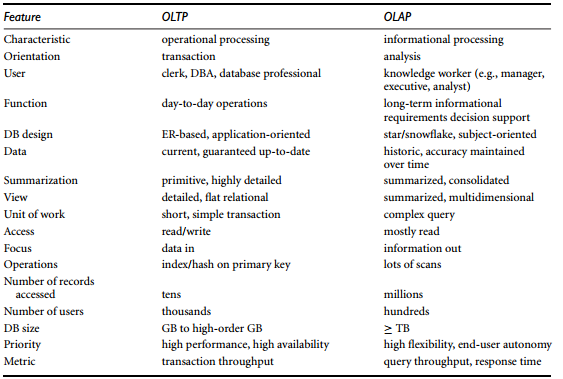
\includegraphics[width=\textwidth]{pics/oltpolap.png}
			\caption{OLTP vs. OLAP}
		\end{figure}

	\clearpage
	\subsection{Data Warehouse Multitier Architecture}

		{\bf "Tier 0" - Raw data:} this is not actually a layer in the data warehouse architecture, 
		but it is the collection of the raw data from operational databases and external sources.

		{\bf Tier 1 - Warehouse database servers:} is almost always a relational database system.
		Back-end tools and utilities are used to feed data into the bottom tier from operational
		databases or other external sources. These tools and utilities perform data extraction
		({\bf gateways}), 
		cleaning, and transformation (e.g., merge similar data from different sources into a 
		uniformed format), as well as load and refresh functions to update data warehouse. 

		{\bf Tier 2 - OLAP server:} typically implemented using either (1) a {\bf relational OLAP (ROLAP)}
		model; or (2) a {\bf multidimensional OLAP (MOLAP)} model. 

		{\bf Tier 3 - Front-end client layer:} contains query and reporting tools, analysis
		tools, and/or data mining tools.

		\begin{figure}[H]
			\centering
			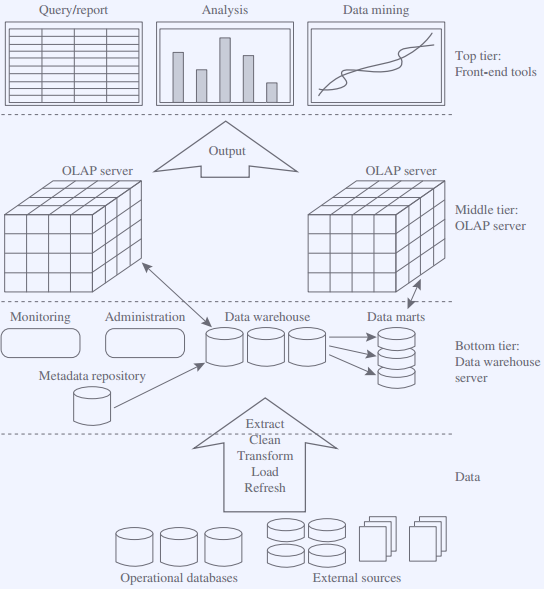
\includegraphics[width=\textwidth]{pics/mutitier.png}
		\end{figure}

	\clearpage
	\subsection{Data Warehouse Models}
		From the architecture point of view, there are three data warehouse models:

		{\bf Enterprise warehouse:} collects all information about subjects spanniing the
		entire organizaiton. It provides corporate-wide data integration, usually from
		one or more operational systems or external information providers, 
		and is cross-functional in scope. 

		{\bf Data mart:} contains subset of corporate-wide data that is one value to
		a specific group users. The scope is confined to specific selected subjects. 
		For example,  a marketing data mart confine its subjects to customer, item, and sales. 
		Depending on the source of data, data marts can be categorized as independent
		or dependent. Independent data marts are sourced from data captured from one
		or more operational systems or external infromation providers.
		Dependent data marts are sourced directly from enterprise data warehouses. 

		{\bf Virtual warehouse:} is a set of views over operational databases.
		For efficiency query processing, only some of the possible summary views may
		be materialized. A virtual warehouse is easy to build but requires excess capacity
		on operational database servers. 

		{\bf Top-down and bottom-up approaches to data warehouse development:}

		{\color{red} viktig ????}

	\subsection{Extraction, Transformation and Loading}

		Data warehouse systems use back-end tools and utilities to populate and refresh
		their data. These tools and utilities include the following functions:

			{\bf Data extraction:} tyically gathers data from multiple, heterogeneous,
			and external sources. 

			{\bf Data cleaning:} detects errors in the data and rectifies them when possible.
			
			{\bf Data transformation:} converts data from legacy or host format to warehouse
			format
			
			{\bf Load:} sort, summarizes, consolidates, computes views, checks integrity, and
			build indices and partitions. 
			
			{\bf Refresh:} propagates the updates from the data sources to the warehouse. 

	\subsection{Metadata Repository}

		{\bf Metadata} are data about data. When used in data warehouse, metadata are the
		data that define warehouse objects. Metadata in data warehouse are included in the
		bottom tire in the data warehousing architecture. A metadata repository should 
		contain the following:

			\begin{itemize}
				\item A description of the data warehouse structure
				\item Operational metadata
				\item The algorithms used for summarization
				\item Mapping from the operational environment to the data warehouse.
				\item Data related to system performance
				\item Business metadata, which include business terms and definitions, data
				ownership information, and charging policies.  
			\end{itemize}

\section{Data Warehouse Modelling: Data Cube and OLAP}
	
	\subsection{Data Cube: A Multidimensional Data Model}

	\subsection{Stars, Snowflakes, and Fact Constellations}

	\subsection{Dimensions - Concept Hierarchies}

	\subsection{Measures}

	\subsection{OLAP Operations}